% Standalone conceptual figure: the heterogeneous population as a Markov chain.
% Style follows rsc/traitors/tex/panel_diagram.tex. Not \input by main.tex.
% Build: pdflatex main.tex
\documentclass[border=4pt]{standalone}
\usepackage{tikz}
\usepackage{amsmath}
\usetikzlibrary{arrows.meta, calc, positioning, backgrounds}

\definecolor{coop}{HTML}{009E73}     % cooperate (Okabe-Ito teal)
\definecolor{defect}{HTML}{D55E00}   % defect    (Okabe-Ito vermillion)
\definecolor{neutral}{HTML}{8C8C8C}
\definecolor{accent}{HTML}{0072B2}   % Okabe-Ito blue
\definecolor{warn}{HTML}{E69F00}

\begin{document}
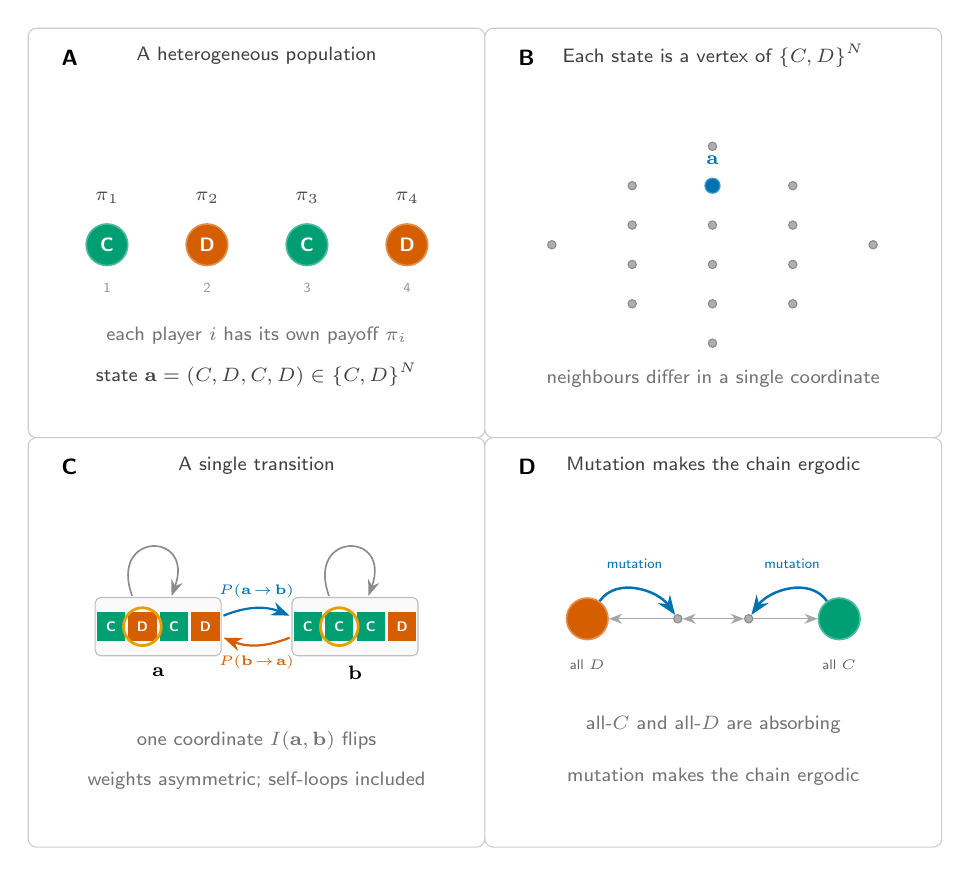
\begin{tikzpicture}[
    >=Stealth,
    font=\sffamily,
    player/.style={circle, minimum size=15pt, inner sep=0pt, line width=0.6pt,
                   font=\sffamily\scriptsize\bfseries, text=white},
    cnode/.style={player, fill=coop, draw=coop!70},
    dnode/.style={player, fill=defect, draw=defect!70},
    sq/.style={rectangle, minimum size=0.36cm, inner sep=0pt, line width=0.5pt,
               font=\sffamily\tiny\bfseries, text=white},
    vtx/.style={circle, fill=neutral!70, draw=neutral, minimum size=3pt,
                inner sep=0pt},
    vhi/.style={circle, fill=accent, draw=accent!70, minimum size=5.5pt,
                inner sep=0pt},
    edge/.style={line width=0.4pt, draw=black!35},
    panellabel/.style={font=\sffamily\footnotesize\bfseries, anchor=north west},
    ptitle/.style={font=\sffamily\scriptsize, text=black!75, align=center},
    note/.style={font=\sffamily\scriptsize, text=black!55, align=center},
]

\def\pw{5.2}
\def\ph{4.6}
\def\gap{0.6}

\coordinate (P1) at (0, \ph+\gap);
\coordinate (P2) at (\pw+\gap, \ph+\gap);
\coordinate (P3) at (0, 0);
\coordinate (P4) at (\pw+\gap, 0);

% Panel A: the general heterogeneous model
\begin{scope}[shift=(P1)]
    \draw[draw=black!20, fill=white, rounded corners=3pt]
        (-0.3,-0.3) rectangle (\pw+0.3, \ph+0.3);
    \node[panellabel] at (0, \ph+0.15) {A};
    \node[ptitle] at (\pw/2, \ph-0.05) {A heterogeneous population};

    \foreach \k/\sty/\lab in {1/cnode/C, 2/dnode/D, 3/cnode/C, 4/dnode/D} {
        \pgfmathsetmacro{\x}{0.7 + (\k-1)*1.27}
        \pgfmathsetmacro{\y}{\ph/2 - 0.15}
        \node[\sty] (pA\k) at (\x,\y) {\lab};
        \node[font=\sffamily\scriptsize, text=black!70] at (\x, \y+0.6) {$\pi_{\k}$};
        \node[font=\sffamily\tiny, text=black!40] at (\x, \y-0.55) {\k};
    }
    \node[note] at (\pw/2, 1.0)
        {each player $i$ has its own payoff $\pi_i$};
    \node[font=\sffamily\scriptsize, text=black!75] at (\pw/2, 0.5)
        {state $\mathbf{a}=(C,D,C,D)\in\{C,D\}^N$};
\end{scope}

% Panel B: the state space (hypercube, by number of cooperators)
\begin{scope}[shift=(P2)]
    \draw[draw=black!20, fill=white, rounded corners=3pt]
        (-0.3,-0.3) rectangle (\pw+0.3, \ph+0.3);
    \node[panellabel] at (0, \ph+0.15) {B};
    \node[ptitle] at (\pw/2, \ph-0.05) {Each state is a vertex of $\{C,D\}^N$};

    % vertices: x = 0.55 + col*1.02 ; y = 2.15 + row*0.50
    \node[vtx] (v0000) at (0.55,2.15) {};
    \node[vtx] (v1000) at (1.57,2.90) {};
    \node[vtx] (v0100) at (1.57,2.40) {};
    \node[vtx] (v0010) at (1.57,1.90) {};
    \node[vtx] (v0001) at (1.57,1.40) {};
    \node[vtx] (v1100) at (2.59,3.40) {};
    \node[vhi] (v1010) at (2.59,2.90) {};
    \node[vtx] (v1001) at (2.59,2.40) {};
    \node[vtx] (v0110) at (2.59,1.90) {};
    \node[vtx] (v0101) at (2.59,1.40) {};
    \node[vtx] (v0011) at (2.59,0.90) {};
    \node[vtx] (v1110) at (3.61,2.90) {};
    \node[vtx] (v1101) at (3.61,2.40) {};
    \node[vtx] (v1011) at (3.61,1.90) {};
    \node[vtx] (v0111) at (3.61,1.40) {};
    \node[vtx] (v1111) at (4.63,2.15) {};

    \begin{scope}[on background layer]
        \foreach \t in {v1000,v0100,v0010,v0001} \draw[edge] (v0000)--(\t);
        \draw[edge] (v1000)--(v1100) (v1000)--(v1010) (v1000)--(v1001);
        \draw[edge] (v0100)--(v1100) (v0100)--(v0110) (v0100)--(v0101);
        \draw[edge] (v0010)--(v1010) (v0010)--(v0110) (v0010)--(v0011);
        \draw[edge] (v0001)--(v1001) (v0001)--(v0101) (v0001)--(v0011);
        \draw[edge] (v1100)--(v1110) (v1100)--(v1101);
        \draw[edge] (v1010)--(v1110) (v1010)--(v1011);
        \draw[edge] (v1001)--(v1101) (v1001)--(v1011);
        \draw[edge] (v0110)--(v1110) (v0110)--(v0111);
        \draw[edge] (v0101)--(v1101) (v0101)--(v0111);
        \draw[edge] (v0011)--(v1011) (v0011)--(v0111);
        \foreach \t in {v1110,v1101,v1011,v0111} \draw[edge] (\t)--(v1111);
    \end{scope}

    \node[font=\sffamily\scriptsize, text=accent, anchor=south] at (2.59,3.05) {$\mathbf{a}$};
    \node[note] at (\pw/2, 0.45)
        {neighbours differ in a single coordinate};
\end{scope}

% Panel C: a single transition
\begin{scope}[shift=(P3)]
    \draw[draw=black!20, fill=white, rounded corners=3pt]
        (-0.3,-0.3) rectangle (\pw+0.3, \ph+0.3);
    \node[panellabel] at (0, \ph+0.15) {C};
    \node[ptitle] at (\pw/2, \ph-0.05) {A single transition};

    % left state a = C D C D
    \draw[rounded corners=2pt, draw=black!25, fill=black!2]
        (0.55,2.13) rectangle (2.15,2.87);
    \foreach \k/\col/\lab in {1/coop/C,2/defect/D,3/coop/C,4/defect/D} {
        \pgfmathsetmacro{\x}{0.75 + (\k-1)*0.4}
        \node[sq, fill=\col] at (\x,2.50) {\lab};
    }
    \node[font=\sffamily\scriptsize] at (1.35,1.92) {$\mathbf{a}$};

    % right state b = C C C D  (player 2 flipped D -> C)
    \draw[rounded corners=2pt, draw=black!25, fill=black!2]
        (3.05,2.13) rectangle (4.65,2.87);
    \foreach \k/\col/\lab in {1/coop/C,2/coop/C,3/coop/C,4/defect/D} {
        \pgfmathsetmacro{\x}{3.25 + (\k-1)*0.4}
        \node[sq, fill=\col] at (\x,2.50) {\lab};
    }
    \node[font=\sffamily\scriptsize] at (3.85,1.92) {$\mathbf{b}$};

    % highlight the differing coordinate (player 2)
    \draw[warn, line width=1pt] (1.15,2.50) circle (0.24);
    \draw[warn, line width=1pt] (3.65,2.50) circle (0.24);

    % directed, asymmetric arrows
    \draw[->, accent, line width=0.8pt] (2.18,2.64) to[out=22,in=158] (3.02,2.64);
    \node[font=\sffamily\tiny, text=accent] at (2.6,2.95) {$P(\mathbf{a}\!\to\!\mathbf{b})$};
    \draw[->, defect, line width=0.8pt] (3.02,2.36) to[out=-158,in=-22] (2.18,2.36);
    \node[font=\sffamily\tiny, text=defect] at (2.6,2.05) {$P(\mathbf{b}\!\to\!\mathbf{a})$};

    % self-loops
    \draw[->, black!45, line width=0.6pt]
        (1.02,2.89) to[out=110,in=70,looseness=4.5] (1.52,2.89);
    \draw[->, black!45, line width=0.6pt]
        (3.52,2.89) to[out=110,in=70,looseness=4.5] (4.02,2.89);

    \node[note] at (\pw/2, 1.05)
        {one coordinate $I(\mathbf{a},\mathbf{b})$ flips};
    \node[note] at (\pw/2, 0.55)
        {weights asymmetric; self-loops included};
\end{scope}

% Panel D: mutation makes the chain ergodic
\begin{scope}[shift=(P4)]
    \draw[draw=black!20, fill=white, rounded corners=3pt]
        (-0.3,-0.3) rectangle (\pw+0.3, \ph+0.3);
    \node[panellabel] at (0, \ph+0.15) {D};
    \node[ptitle] at (\pw/2, \ph-0.05) {Mutation makes the chain ergodic};

    % the two absorbing corners of the state space (cf. panel B)
    \node[dnode] (allD) at (1.0,2.6) {};
    \node[vtx]   (m1)   at (2.15,2.6) {};
    \node[vtx]   (m2)   at (3.05,2.6) {};
    \node[cnode] (allC) at (4.2,2.6) {};
    \node[font=\sffamily\tiny, text=black!60, anchor=north] at (1.0,2.2) {all $D$};
    \node[font=\sffamily\tiny, text=black!60, anchor=north] at (4.2,2.2) {all $C$};

    % ordinary moves drift towards fixation
    \draw[edge, ->] (m1)--(allD);
    \draw[edge, <->] (m1)--(m2);
    \draw[edge, ->] (m2)--(allC);

    % mutation lets the chain escape the absorbing corners
    \draw[->, accent, line width=0.9pt] (allD) to[out=55,in=125] (m1);
    \draw[->, accent, line width=0.9pt] (allC) to[out=125,in=55] (m2);
    \node[font=\sffamily\tiny, text=accent] at (1.6,3.3) {mutation};
    \node[font=\sffamily\tiny, text=accent] at (3.6,3.3) {mutation};

    \node[note] at (\pw/2, 1.25)
        {all-$C$ and all-$D$ are absorbing};
    \node[note] at (\pw/2, 0.6)
        {mutation makes the chain ergodic};
\end{scope}

\end{tikzpicture}
\end{document}
